\section{Regularization}\label{sec:regularization}

With the advent of modern computing resources researchers gained the ability to operate very complex models giving rise to the problem of over-fitting. Consequentially while performance on the data the model is fit to increases, it rapidly deteriorates outside that region. As much of current research deals with somehow bridging the barriers between different regions of data, or entirely different distributions, reducing the chance of a model over-fitting is crucial in most applications. In this thesis we tackle data that come from multiple different instances of the same nuclear-experiment, which means training on one instance should translate to another. Additionally it is greatly beneficial if the recognition of reactions translate between different experiments.   

Finding measures to reduce over-fitting has been a goal for machine learning researchers for near on $50$ years. The first modern breakthrough was adding a constraint on the cumulative magnitude of the coefficients to linear regression systems. This form of restriction proved hugely beneficial for the simple reason that it restricted the models ability to express all of its complexity. Introduced in 1970 by \citet{Hoerl1970} the addition of a $L_2$ norm-constraint to linear regression was dubbed \textit{ridge} regression. Experiments with different norms were carried out in the years following the elegant discovery by \cite{Hoerl1970}. Perhaps most influential of them is the use of the $L_1$-norm, first successfully implemented by \citet{Tibshirani1996}. As the norms have different geometric expressions the consequence of their addition to the cost was evident in the types of solutions generated by their inclusion. We illustrate this geometry in figure \ref{fig:regularization}, copied from \cite{Mehta2019}, where the lasso penalty is shown to result in a constrained region for the parameter inside a region with vertices pointing along the feature axes. Intuitively this indicates that for a $L_1$ penalty the optimal solution is a sparse one where as many parameters as possible are zero while still minimizing cost. For $L_2$ ridge regression these vertices are not present and the region has an even boundary along the feature axes resulting in solutions where most parameter values are small. The figure is made using the understanding that adding a regularization term is equivalent to solving a constrained optimization problem, for example in the case of least squares regression 

\begin{align}
\theta^* = \argmin_{||\theta||_2^2<t} ||y_i - f(\mathbf{x}_i; \theta)||_2^2.
\end{align}

\begin{figure}
\centering
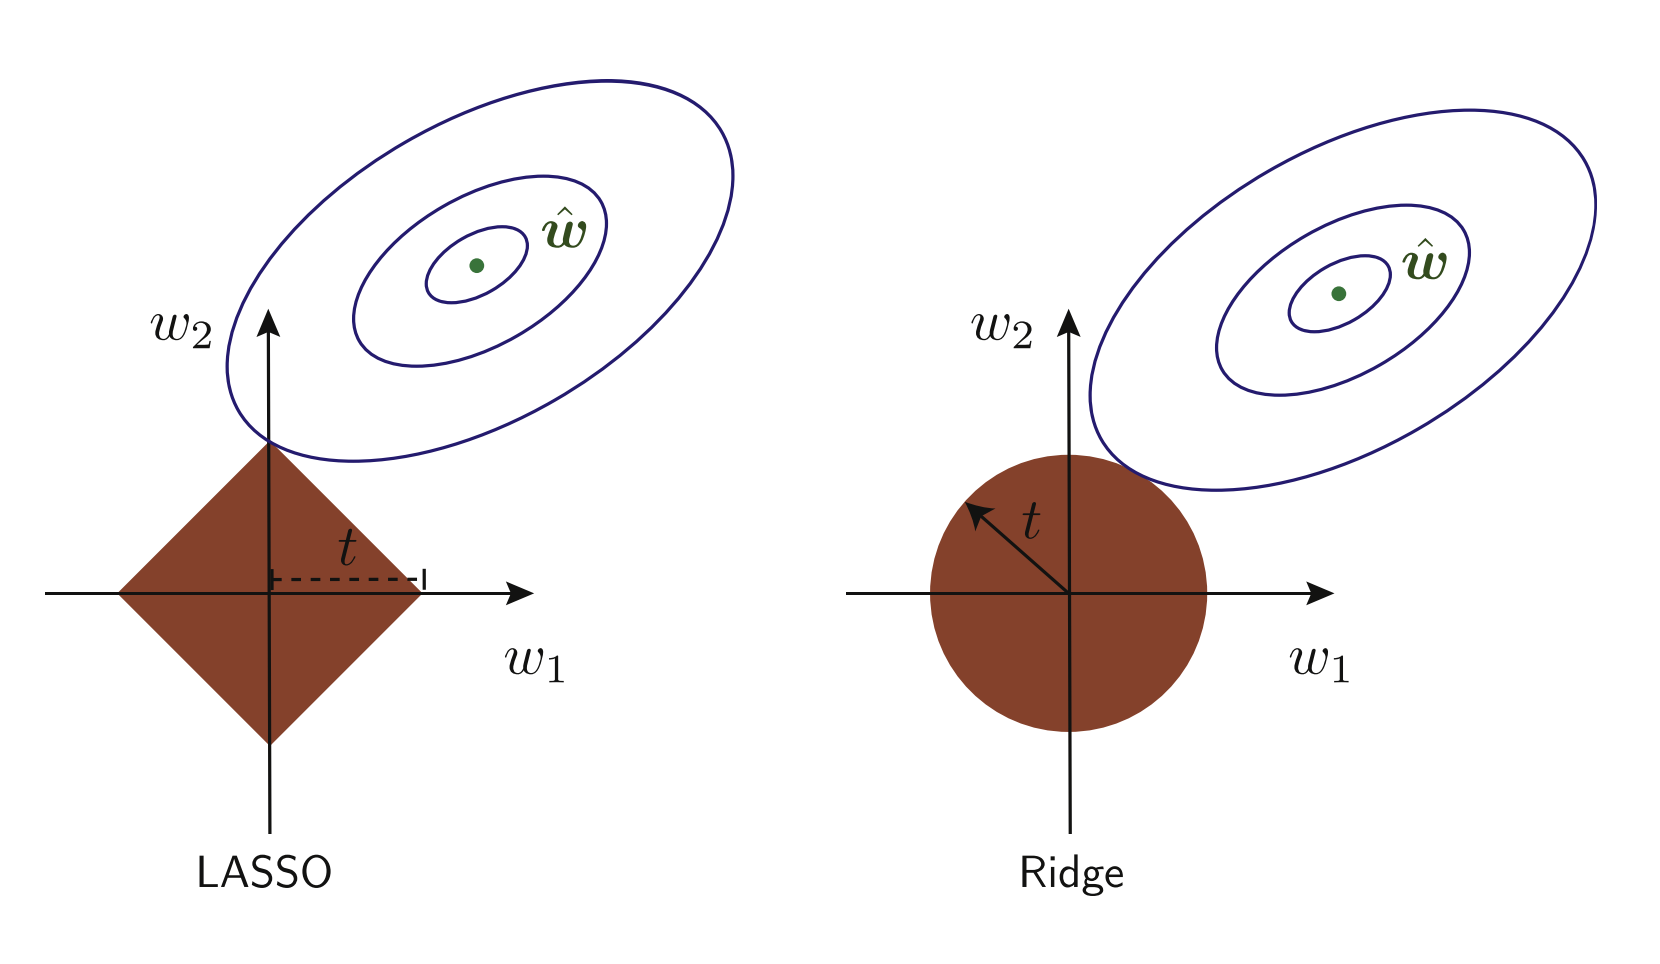
\includegraphics[width=\textwidth]{../figures/regularization}
\caption[Geometric interpretation of the $L_1$ and $L_2$ regularization and the squared error cost]{Demonstrating the effect of a regularization constraint on a 2-variable optimization. The blue ovals represent the squared error, as it is quadratic in the parameters $w_i$. And the shaded brown region represents the restriction on the values of $w_i$, s.t. the only eligible values for the parameters are inside this region. Since the $L_1$ norm has these vertices on the feature axis we expect that the contour of the cost will touch a vertex consequently generating a sparse feature representation. The $L_2$ norm does not have these protrusions and will then generally intersect with the cost-contour somewhere that generates a linear combination of features that all have small coefficients. Figure copied from \citet{Mehta2019}, which in turn adapted a figure from Friedman et al. (2001)}\label{fig:regularization}
\end{figure}

The inclusion of an $L_1$-norm to the linear regression cost-function proved to be challenging as had no closed form solution and thus required iterative methods like gradient descent, described in detail in section \ref{sec:gd}. 

We still have to show how these additional contributions add to the cost-function. We begin by defining the general $L_p$ norm of a vector $\mathbf{x} \in \mathcal{R}^n$ as

\begin{equation}
L_p(\mathbf{x}) = \left(\sum |x_i|^p\right)^{\frac{1}{p}}.
\end{equation}

\noindent A common notation for the $L_p(\cdot)$ norm that we will also use in this thesis is $L_p(\cdot) = ||\cdot||_p$. We note that the familiar euclidian distance is just the $L_2$ norm of a vector difference. Wile the $L_1$ term is commonly called the Manhattan or taxicab-distance, aptly named as one can think of it as the length of the city blocks a cab-driver drives from one house to another.

Modifying the cost function then is as simple as adding the normed coefficients. To demonstrate we add a ridge regularization term to the squared error cost with $\lambda$ determining the strength of the regularization while the rest of the symbols have their usual meaning

\begin{equation}\label{eq:mse_ridge}
C(\hat{y}_i, f(\mathbf{x}_i; \theta)) = (\hat{y}_i - f(\mathbf{x}_i; \theta))^2 + \lambda\sum|\theta_i|^2.
\end{equation}

\noindent Assuming now that the model $f$ is a linear regression model we can derive the solution by substituting in the model from section \ref{sec:LinReg} and repeating the procedure of taking the derivative with respect to the parameters. We begin by substituting in and taking the derivative 

\begin{align}
C(\mathbf{\hat{y}}, \mathbf{Xw}) &= ( \mathbf{\hat{y}} - \mathbf{Xw})^T( \mathbf{\hat{y}} - \mathbf{X}^T\mathbf{w}) - \lambda \mathbf{w}^T\mathbf{w}, \\
\nabla_\mathbf{w} C &= -2\mathbf{X}^T\mathbf{\hat{y}} + 2\mathbf{X}^T\mathbf{Xw} - 2\lambda\mathbf{w}. 
\end{align}
\noindent Following from the section on linear regression to find the optimal parameters we find the zero intersection of the derivative and solve for the parameters 

\begin{align}
\mathbf{0} &=  -\mathbf{X}^T\mathbf{\hat{y}} + (\mathbf{X}^T\mathbf{X} - \lambda \mathbf{I})\mathbf{w}, \\
\mathbf{w} &= (\mathbf{X}^T\mathbf{X} - \lambda \mathbf{I})^{-1}\mathbf{X}^T\mathbf{\hat{y}}.
\end{align}

\noindent The solution is very close to that of the ordinary least squares problem with an added term in the matrix inversion. This addition turns out to be very convenient as it ensures the resulting matrix has full rank, which avoids some of the potential problems when trying to estimate the inverse. 

Conceptually the regularization term added to the cost function modifies what parameters satisfy the $\argmin$ in equation \ref{eq:cost} by adding a penalty to parameters having high values. This is especially useful in cases where features are co-variate or the data is noisy. 
Regularization then reduces the probability of overfitting by limiting the expressed complexity of a model. In the example of polynomial regression lasso regularization forces many of the coefficients to be zero-valued in such a way that it still performs maximally. \todo{add subsection on dropout and batchnorm} 


\subsection{Batch Normalization}\label{sec:batchnorm}
\todo{maybe dropout?}